\subsection{Modalanalyse (omega, modeshape, måling med mobil/frequency, FFT)} 

Modalanalysen inngår som en del av studien av konstruksjoners dynamiske egenskaper og oppførsel. Begrepet henger følgelig tett sammen med det overordnet temaet ``structural dynamics'', eller konstruksjonsdynamikk på norsk. Med egenskaper menes her egenfrekvenser, dempingskoeffisienter og modeformer (engelsk: \emph{mode shapes}). I påfølgende underkapitler skal vi introdusere kort om egenfrekvenser og modeformer.

\subsection{Egenfrekvenser}
For å forklare hva som menes med egenfrekvenser (flertall) til en konstruksjon, bør vi starte med å forklare hva én egenfrekvens (entall) er. På engelsk skiller man mellom begrepene \emph{circular frequncy} $\omega$, og \emph{cyclic frequency} $f$ (Hz), som hhv. kan oversettes til vinkelhastighet og frekvens på norsk. Begrepene går gjerne litt om hverandre i talen, men forskjellen er bare en faktor på $2\pi$. Der vinkelhastighet $\omega$ måles i radianer/sekund, måles frekvens $f$ i syklus/sekund (Hz). En syklus er hele ``runden'' konstruksjon tar fra ingen forskyvning til mest ytterligende forskyvning ($\pi/2$ radianer), tilbake til utgangsposisjon ($\pi$ radianer), til mest ytterligende forskyvning på ``motsatt'' side ($3\pi/2$ radianer) og tilbake til utgangsposisjonen ($2\pi$ radianer).  Sammenhengen er $\omega = 2 \pi f$, men vi kommer nærmere inn på dette når $\omega$-verdiene til en konstruksjon utledes. \\

En vanlig måte å introdusere konseptet om egenfrekvenser på er å tegne opp en enkel konstruksjon som kun har èn frihetsgrad \parencite{CE809_FreeVibrationResponseOfSDFSystems}. Vi kaller konstruksjonen enkel fordi den ``\emph{..can be idealized as a concentrated or lumped mass \emph{m} supported by a massless structure with stiffness \emph{k} in the lateral direction} \parencite[s. 3]{Chopra2019-da}. I dette tilfelle en en-etasjers bygning med et voldsomt betongtak, og all massen antas altså å være plassert/konsentrert på taket (engelsk: \emph{lumped mass}). Bygget er innspent mot bakken, og vi ser bort fra demping som konstruksjonen måtte ha. I realiteten vil ha alle ha noe demping pga. f. eks friskjon mellom ulike konstruksjonselementer, men for å forstå egenfrekvensbegrepet (og senere modeformer), kan vi sette dempingskoeffisient $c=0$ \parencite[]{CE809_FreeVibrationResponseOfSDFSystems}. På figur \ref{fig:Enkel idealisert konstruksjon: én frihetsgrad} tenkes massen konsentrert i den blå sirkelen. At den har én frihetsgrad betyr her at det kun tillates én forskvyning/rotasjon. Her får forskvyningen $u$ gå langs aksen $x$:

\begin{figure}[h]
    \centering
    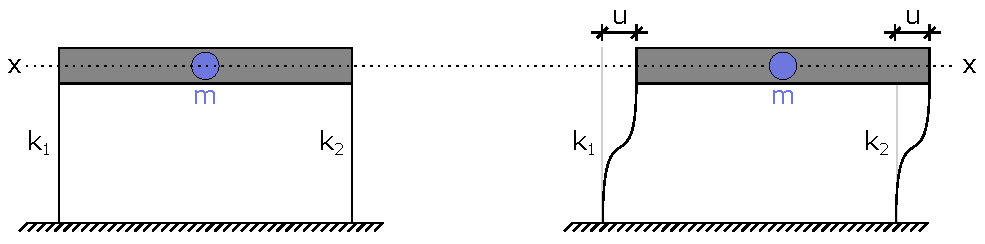
\includegraphics[width=\linewidth]{0 FIGURER/SDOF.pdf}
    \caption{Enkel idealisert konstruksjon: én frihetsgrad}
    \label{fig:Enkel idealisert konstruksjon: én frihetsgrad}
\end{figure}

De masseløse søylene bidrar med en total stivhet $k = k_1 + k_2$ mot denne forskyvningen. Hvis vi tenker oss at konstruksjonen utsettes for en harmonisk kraft over tid, så får vi følgende bevegelsesligning for vår konstruksjon: 

\begin{equation}
    m \ddot{u} + ku = p_0 \sin \lrp{\omegabar t}
\end{equation}

der $m$ er massen, $\ddot{u}$ er dobbeltderiverte til forskyvningen med hensyn på tid (akselerasjon), $k$ er stivhet mot forskyvning langs $x$, $p_0$ er amplituden til den påførte, harmoniske kraften og $\omegabar$ er den påførte kraftens egenfrekvens/vinkelhastighet (engelsk: \emph{forcing freqeuency}). Fra matematikken kjenner vi igjen dette som en andreordens, inhomogen differensialligning. Den har en kjent løsning, og består av summen av den homogene løsningen og den partikulære løsningen. \\

\textbf{Homogen løsning
} \quad Bevegelsesligningen for udempet konstruksjon i fri vibrasjon, én frihetsgrad:

\begin{equation} \label{eq: SDOF_FreeVib}
    m \ddot{u} + ku  = 0 
\end{equation}

Gjetter løsning på formen $u = e^{rt}$, og setter inn i \eqref{eq: SDOF_FreeVib}: 

\begin{equation}
    mr^2e^{rt} + ke^{rt} = 0 \longrightarrow  \underbrace{e^{rt}}_{\neq 0} \lrp{mr^2 + k} = 0 \longrightarrow r = \pm \sqrt{-\frac{k}{m}} = 0 \pm \sqrt{\frac{k}{m}}i
\end{equation}

Her setter vi $\omega_n = \sqrt{\frac{k}{m}}$, og ser at $r$ får to løsninger: $r_1 = 0 + \omega_n i$ og $r_2 = 0 - \omega_n i$. Dette er et komplekskonjugert par, som har kjent løsning:

\begin{equation} \label{eq:u(t)SDOF_FreeVib}
    u(t) = e^{0t}\Bigl(A \cos \lrp{\omega_n t} + B \sin \lrp{\omega_n t}\Bigr) = A \cos \lrp{\omega_n t} + B \sin \lrp{\omega_n t}
\end{equation}

hvor $\omega_n$ er den udempede konstruksjonens vinkelhastighet! Som nevnt i innledningen av dette underkapitlet er dens størrelse målt i radianer per sekund, og kan kan skrives som $\omega_n =  2\pi f$, der $f$ er konstruksjonens frekvens (Hz). Dender konstantene $C_1$ og $C_2 $ bestemmes av initialbetingelsene $u(0)$ og $\dot{u}(0)$.  Da får vi $A = u(0)$ og $B = \frac{\dot{u}(0)}{\omega_n}$. Videre skriver vi om til formen $\rho \sin \lrp{\omega_n t+ \theta}$. Vi utnytter den kjente trigonometriske identiteten for en vinkelsum i sinus-funksjon:

\begin{equation} \label{eq:SumAvVinklerSinurs}
    \rho \sin \lrp{\omega_n t+ \theta} = \rho \Bigl(\sin \lrp{\omega_n} \cos \lrp{\theta} + \cos \lrp{\omega_n t} \sin \lrp{\theta} \Bigr)
\end{equation}

Hvis vi sammenligner koeffisientene med $A$ og $B$ i ligning \eqref{eq:u(t)SDOF_FreeVib} får vi:

\begin{equation} \label{eq:KoeffisienterSinCos}
    A = \rho \sin \lrp{\theta}, \qquad B = \rho \cos \lrp{\theta}
\end{equation}

Ved å kvadrere begge ligningene, og ta kvadratroten av summen får vi:

\begin{equation} \label{eq:rhoSDOFFreeVib}
    \sqrt{A^2 + B^2} = \sqrt{\rho^2 \Bigl({\sin^2\lrp{\theta} + \cos^2\lrp{\theta}\Bigr)}} = \rho
\end{equation}

Ved å ta $\arctan$ av kvotienten på begge sider får vi:

\begin{equation} \label{eq:arctan}
    \arctan \lrp{\frac{A}{B}} = \arctan \lrp{\frac{\rho \sin \lrp{\theta}}{\rho \cos \lrp{\theta}}} = \arctan \lrp{\tan \lrp{\theta}} = \theta
\end{equation}

Den homogene løsninga til denne andreordens differensialligningen blir: 

\begin{equation} \label{eq: AndreOrdensDiffLigning}
    u(t) = \underline{\rho \sin \lrp{\omega_n t + \theta}} \quad \text{hvor:} \quad \rho = \sqrt{\lrp{(u(0)}^2 + \lrp{\frac{\dot{u}(t)}{\omega_n}}^2}, \quad \theta = \arctan \lrp{\frac{u(0)}{\dot{u}(0) / \omega_n}}
\end{equation}